\documentclass{article}

\usepackage{amsmath}
\usepackage{amssymb}
\usepackage{algorithm}
\usepackage[noend]{algpseudocode}		% for algorithms in pseudo code. Usage: \begin{algorithmic}
\MakeRobust{\Call}
\usepackage{tikz}	% for diagrams
\usetikzlibrary{positioning}
\usetikzlibrary{quotes}

\setlength{\parskip}{\smallskipamount}

\title{Analysis of Algorithms \\
\medskip
\large Homework 4}
\author{Abraham Murciano}

\begin{document}

\maketitle

\section{Dijkstra's Algorithm with negative weights}

\subsection*{Part A}

Figure \ref{q1a} shows a graph with negative weights such that if we apply Dijkstra's algorithm to find the shortest path between vertices \(S\) and \(D\), it will return the wrong path.

\begin{figure}[h]
	\centering
	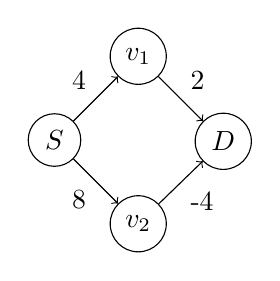
\begin{tikzpicture}
		[vertex/.style={circle, draw=black, node distance=0.8cm}]
		\node[vertex] (S) {\(S\)};
		\node[vertex, above right=of S] (v1) {\(v_1\)};
		\node[vertex, below right=of S] (v2) {\(v_2\)};
		\node[vertex, below right=of v1] (D) {\(D\)};
		\draw[->] (S) to["4"] (v1);
		\draw[->] (S) to["8" below left] (v2);
		\draw[->] (v1) to["2"] (D);
		\draw[->] (v2) to["-4" below right] (D);
	\end{tikzpicture}
	\caption{Graph for which Dijkstra doesn't work}
	\label{q1a}
\end{figure}

\end{document}